\subsubsection{\gls{KA}}

\textbf{Ansvar} \\
Kasseapparatet er den del af systemet hvor produktkataloget bliver vist og benyttet til salg af produkter. Her laves kvitteringer og der bliver vist en liste/indkøbskurv med de produkter som en evt. kunde ønsker at købe. Produktkataloget bliver hentet ved en forespørgsel til Centralserver og kasseapparatet ved derved intet om oprettelse og redigering af de produkter som den fremviser. \\

\textbf{Sekvensdiagram}
\begin{figure}[H]
	\centering
	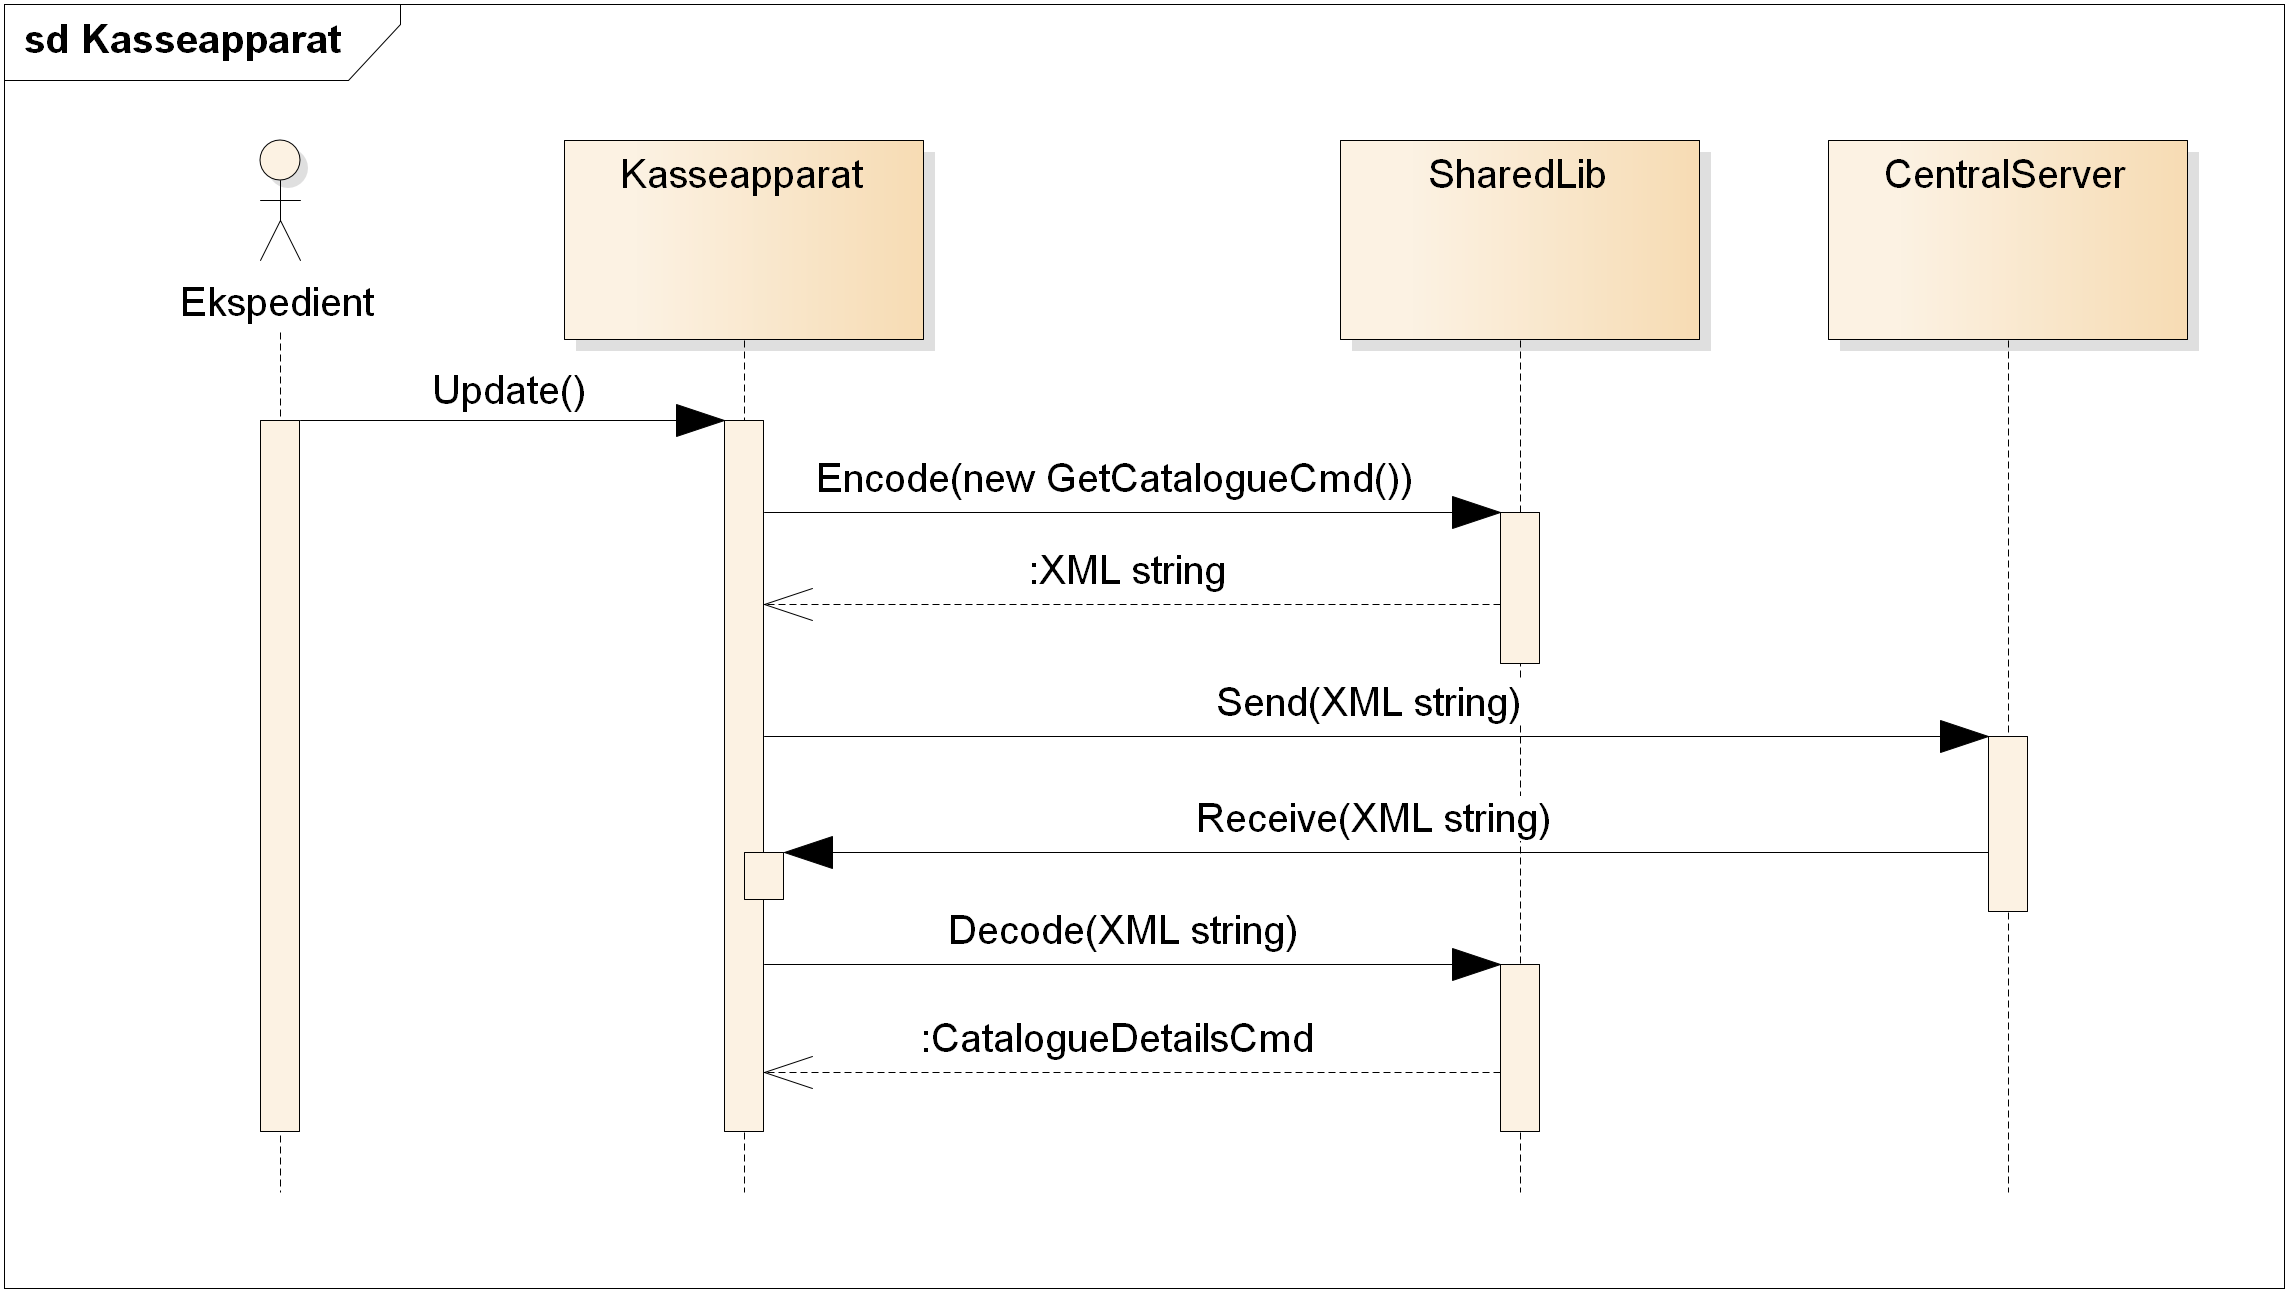
\includegraphics[scale=0.7]{Systemarkitektur/LogiskView/Kasseapparat-sekvensdiagram}
	\caption{Sekvensdiagram for kommunikation mellem \gls{KA} og andre pakker}
	\label{fig:logview_kasse_sekvensdiagram}
\end{figure}

Sekvensdiagrammet viser hvordan kasseapparatet kommunikerer med de andre pakker i systemet. Kasseaparatet kommunikerer udelukkende med Centralserver. Når kasseapparatet skal sende en besked til Centralserver bruger den SharedLib til at konvertere et kommandoobjekt til XML og sender herefter denne til Centralserveren. Centralserveren sender derefter en XML-besked tilbage som så derefter bliver omskrevet til et kommandoobjekt, igen ved brug af SharedLib.

\newpage
